% $Header: /cvsroot/latex-beamer/latex-beamer/examples/beamerexample2.tex,v 1.8 2004/10/11 16:10:11 tantau Exp $

% This file is included by beamerexample2.article.tex and
% beamerexample2.beamer.tex 

% Copyright 2003 by Till Tantau <tantau@cs.tu-berlin.de>.
%
% This program can be redistributed and/or modified under the terms
% of the LaTeX Project Public License Distributed from CTAN
% archives in directory macros/latex/base/lppl.txt.

%
% The purpose of this example is to demonstrate the usage of the
% nameslide command
%

\mode<article>
{
  \usepackage{fullpage}
  \usepackage{hyperref}
  \setjobnamebeamerversion{oss-and-search.beamer}
}

\mode<presentation>
{
  \usetheme{Dresden}

  \setbeamercovered{transparent}
}

\usepackage{graphicx}
\usepackage[latin1]{inputenc}
\usepackage[english]{babel}

\title{Open Source and Search}
\author{Paul~Pham}
\date{2 May 2006}
\subject{Presentation Programs}

\institute[UW CSE]{
  University of Washington\\
  Computer Science and Engineering}

\begin{document}

\frame{\maketitle}

%%%%%%%%%%%%%%%%%%%%%%%%%%%%%%%%%%%%%%%%%%%%%%%%%%%%%%%%%%%%%%%%%%%%%%%%%%%%%%%
\section{Overview}

%------------------------------------------------------------------------------
\frame[label=overview]{

  \frametitle{Overview}

  \begin{itemize}
  \item Open Source Software (OSS)
  \item The Social Web
  \item Internet Search
  \item How are they related
  \item Wild speculations about the future of search
  \end{itemize}

}

%%%%%%%%%%%%%%%%%%%%%%%%%%%%%%%%%%%%%%%%%%%%%%%%%%%%%%%%%%%%%%%%%%%%%%%%%%%%%%%
\section{Open Source Software}

%------------------------------------------------------------------------------
\frame[label=sw-model]{

  \frametitle{The Desktop Software Model}

  \begin{figure}[hbt]
  \begin{center}
  \begin{tabular}{lll}
     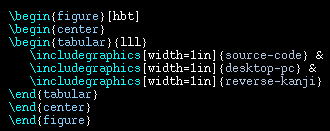
\includegraphics[width=1in]{source-code} &
     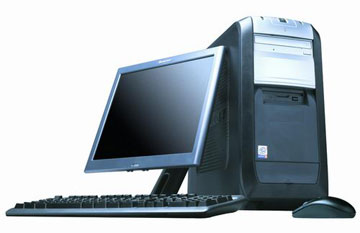
\includegraphics[width=1in]{desktop-pc} &
     
\includegraphics[width=1in]{reverse-kanji}
  \end{tabular}
  \end{center}
  \end{figure}

  \begin{itemize}
  \item The release cycle: Lather, rinse, repeat
  \begin{enumerate}
  \item Developers write program in source code.
  \item Users buy/download and use compiled binaries.
  \item Users send feedback to developers, who incorporate into next release.
  \end{enumerate}
  \item Users and developers are separate.
  \item Everyone interacts with their own machine.
  \end{itemize}
}

%------------------------------------------------------------------------------
\frame[label=sw-closed]{

  \frametitle{Closed Source Software - The Cathedral}

  \begin{figure}[hbt]
  \begin{center}
  \begin{tabular}{lll}
     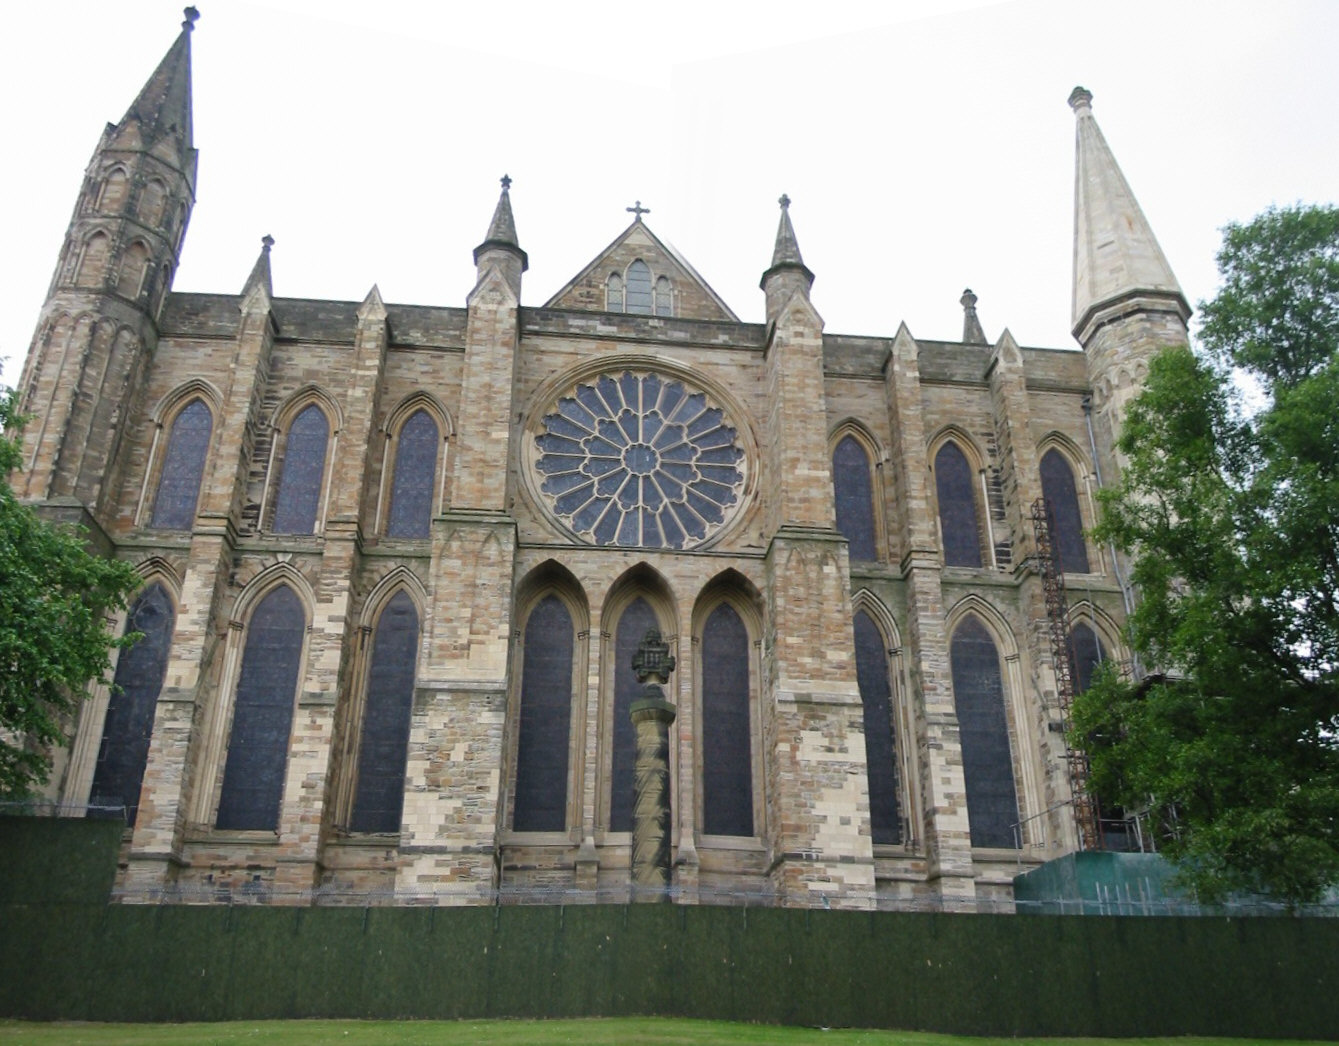
\includegraphics[width=1in]{cathedral-durham} &
     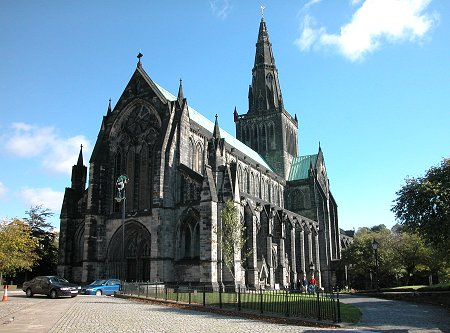
\includegraphics[width=1in]{cathedral-glasgow} &
     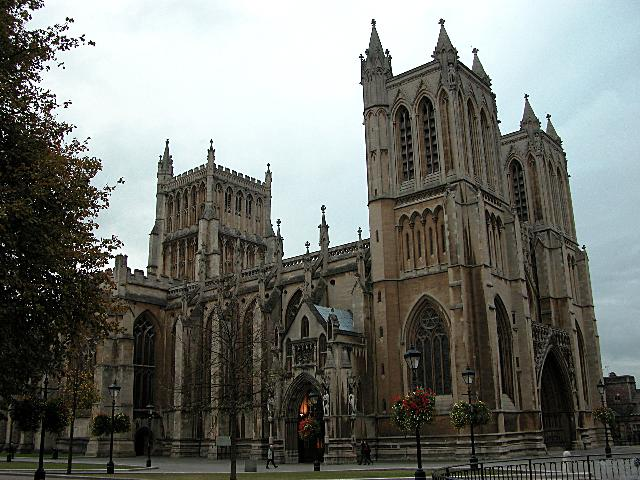
\includegraphics[width=1in]{cathedral-bristol}
  \end{tabular}
  \end{center}
  \end{figure}

  \begin{itemize}
  \item Source code is kept secret, often duplicated.
  \item Development is centralized and done by experts/pros.
  \item Problems are concealed, no guarantee of fixes.
  \item Software is a product, connected to the business.
  \item Success is determined by profit.
  \end{itemize}
}

%------------------------------------------------------------------------------
\frame[label=sw-open]{

  \frametitle{Open Source Software - The Bazaar}

  \begin{figure}[hbt]
  \begin{center}
  \begin{tabular}{lll}
     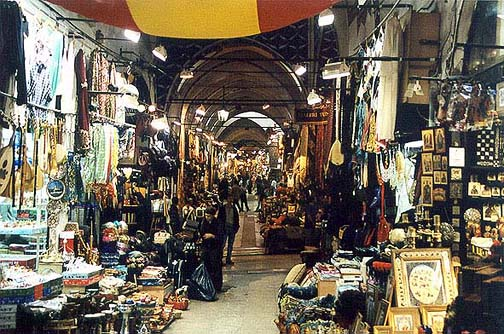
\includegraphics[width=1in]{bazaar} &
     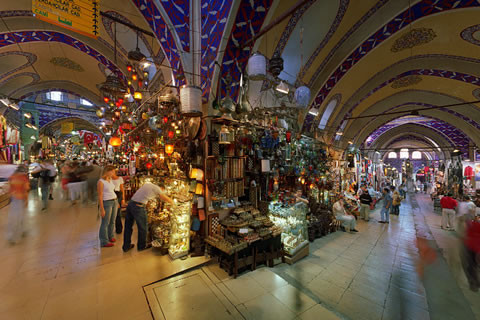
\includegraphics[width=1in]{grand-bazaar} &
     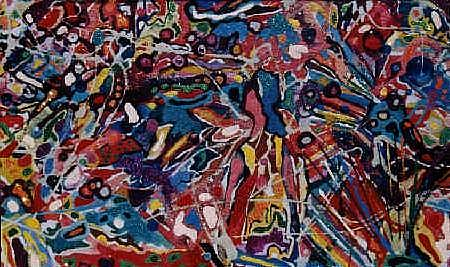
\includegraphics[width=1in]{bizarre-bazaar}
  \end{tabular}
  \end{center}
  \end{figure}

  \begin{itemize}
  \item Source code is freely available, effort is shared.
  \item Development is decentralized and done by anyone (experts and amateurs).
  \item Problems are discovered through independent review.
  \item Support is a service, freedom to fork.
  \item Success is determined by users and actual practice.
  \end{itemize}
}

%------------------------------------------------------------------------------
\frame[label=sw-social]{

  \frametitle{Social Concerns of Open Source}

  \begin{itemize}
  \item Privacy - does it revealing personal information about me?
  \item Truthfulness - does it work the way it claims?
  \item Personalization - can I make it work the way I want? (``scratching an itch'')
  \item Independence - am I free to switch software and still access my data?
  \item Cost - am I paying for what I want?
  \end{itemize}

  OSS can answer positively on all counts.
}

In September 2005, the Peru passed a law mandating that all government
software for handling and storing citizen data must use open standards.
The rationale given was that citizens had a right to access their own data
without being required to purchase software from a particular company.
A protest letter from Microsoft general manager Juan Alberto Gonzalez 
attempted to fill
Peruvian legislators with fear, uncertainty, and doubt (FUD) but Congressman
Edgar Villanueva Nu�ez wrote an incisive response which included the
argument of cost below.

A big problem with closed source software that is sold commercially is that
the consumer price is not connected to the company cost. Empirically
95\% of the software
written in the U.S. is not for sale, but is used in-house. For example, most
software is specialized for a particular bank, insurance company, and 
accounting departments may need specialized
software that is integrated into a particular environment and hard to
reuse.evelop payroll software to serve clients better,
or an IT (information technology) department might write software for
sending e-mail. However, they would not intend to sell it and would just as
easily buy/use something already available if it met their needs.

%------------------------------------------------------------------------------
%\frame[label=sw-economic]{

%%   \frametitle{Open source addresses economic concerns}

%%   \begin{itemize}
%%   \item Security - how can you protect something that's out in the open?
%%   \item Profit - how can you make money if you give the code away?
%%   \item Competition - doesn't this put programmers out of a job?
%%   \end{itemize}
%% }

%------------------------------------------------------------------------------
\frame[label=sw-success]{

  \frametitle{Open Source Success Stories}

  \begin{figure}[hbt]
  \begin{center}
  \begin{tabular}{lllll}
     
\includegraphics[height=0.6in]{tux-logo} &
     
\includegraphics[height=0.6in]{bsd-daemon-hammer} &
     
\includegraphics[height=0.6in]{apache-logo} &
     
\includegraphics[height=0.6in]{apple-logo} &
     
\includegraphics[height=0.6in]{firefox-logo}
  \end{tabular}
  \end{center}
  \end{figure}

  \begin{itemize}
  \item BSD - Solaris, Mac OS X, Windows
  \item Apache - runs 54\% of the world's websites (Netcraft)
  \item Mozilla - Firefox and Thunderbird.
  \item Linux - RedHat, SuSE, Novell, Debian, Ubuntu.
  \item Companies that invest in OSS: IBM, Oracle, Novell
  \item Companies that use OSS: Amazon, eBay, Yahoo!, Google
  \end{itemize}
}

%------------------------------------------------------------------------------
\frame[label=sw-dis]{

  \frametitle{Disadvantages of Open Source}

  \begin{itemize}
  \item Notoriously hard to use (UI is ugly).
  \item Not available for high-end, specialized applications (video editing, photo manipulation).
  \item Bad for entertainment content (movies and music).
  \item Games are different (plugins, mods, open source engines, etc.)
  \item So how can we become beautiful, rich, and famous by using OSS?
  \end{itemize}
}

%% %------------------------------------------------------------------------------
%% \frame[label=sw-indirection]{

%%   \frametitle{Indirection}

%%   \begin{itemize}
%%   \item ``All problems in CS can be solved by indirection.''-- Knuth.
%%   \item Indirection is basically taking a step back.
%%   \item Not many users want to modify OSS, but still want to tweak.
%%   \item How is code controlled? API (application programming interface)
%%   \item Ex: plugins, interfaces, and surrounding communities
%%   \item Indirection again: how will the user use the interface? what kinds of data?
%%   \item Lead into Web 2.0.
%%   \end{itemize}
%% }

%%%%%%%%%%%%%%%%%%%%%%%%%%%%%%%%%%%%%%%%%%%%%%%%%%%%%%%%%%%%%%%%%%%%%%%%%%%%%%%
\section{The Social Web}

%------------------------------------------------------------------------------
\frame[label=web2-intro]{

  \frametitle{The Social Web (Web 2.0)}

  \begin{itemize}
  \item Low-key user content - Craigslist
  \item Reputation mechanisms - eBay ratings
  \item Blogs - Blogger, LiveJournal
  \item Tagging (folksonomy) - Delicious, Flickr
  \item Wikis - Wikipedia, FAQs
  \item Podcasts
  \item Syndication (RSS)
  \item Social networking - MySpace, Friendster, Orkut
  \item Web Platform (GMail/Calendar vs. Outlook)
  \end{itemize}
}

%------------------------------------------------------------------------------
\frame[label=web2-longtail]{

  \frametitle{Chris Anderson's Long Tail}

\begin{figure}[hbt]
  \input{gaussian}
  \centerline{\box\graph}
\end{figure}

  \begin{itemize}
  \item Traditional markets are mediated geographically.
  \item Business target the mainstream (average under a normal curve).
  \item Dissipated communities have no voice.
  \item Internet user participation and automation make niche markets profitable.
  \item Success stories: Amazon reader lists and recommendations, Netflix
  \end{itemize}
}

%------------------------------------------------------------------------------
\frame[label=web2-powerlaw]{

  \frametitle{Ross Mayfield's Power Law of Participation}

  \begin{figure}[hbt]
  \begin{center}
     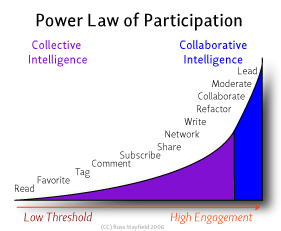
\includegraphics[width=2in]{powerlaw}
  \end{center}
  \end{figure}

  \begin{itemize}
  \item Spectrum of ``group'' intelligence for Social Web.
  \item Also a long tail here to exploit.
  \end{itemize}
}

%------------------------------------------------------------------------------
\frame[label=web2-concern]{

  \frametitle{Report Card of the Social Web}

  \begin{itemize}
  \item Privacy - no (privacy policies)
  \item Truthfulness - no (privacy policies)
  \item Personalization - yes
  \item Independence - yes
  \item Cost - yes
  \end{itemize}

  Questions?
  \begin{itemize}
  \item Do we need more ideas from OSS?
  \item Is the Social Web useful for search?
  \end{itemize}


}

%%%%%%%%%%%%%%%%%%%%%%%%%%%%%%%%%%%%%%%%%%%%%%%%%%%%%%%%%%%%%%%%%%%%%%%%%%%%%%%
\section{Search}

%------------------------------------------------------------------------------
\frame[label=search-weakness]{

  \frametitle{Current Weaknesses of Search}

  \begin{figure}[hbt]
  \begin{center}
     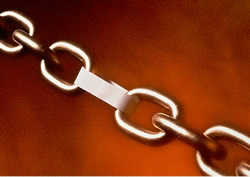
\includegraphics[width=1.5in]{weak-link}
  \end{center}
  \end{figure}

  \begin{itemize}
  \item Dynamically generated websites (online databases).
  \item Multimedia files (video, sound, images)
  \item ``Islands'' of content with no external links.
  \item Personalized search and training.
  \item Search engine optimization (SEO) and spam.
  \end{itemize}
}

%------------------------------------------------------------------------------
\frame[label=search-trends]{

  \frametitle{Recent Search Trends}

  \begin{figure}[hbt]
  \begin{center}
  \begin{tabular}{lll}
     
\includegraphics[width=1in]{google-sitemap} &
     
\includegraphics[width=1in]{google-base} &
     
\includegraphics[width=1in]{google-maps}
  \end{tabular}
  \end{center}
  \end{figure}

  \begin{itemize}
  \item User submission: Google SiteMap
  \item User content and tagging: Google Base (Craigslist clone)
  \item Provides web services through open APIs (maps, search, etc.)
  \item Personalized search (privacy concerns)
  \item Censorship issues (truthfulness concerns)
  \end{itemize}
}

%------------------------------------------------------------------------------
\frame[label=search-google]{

  \frametitle{Open Source and Google}

  \begin{figure}[hbt]
  \begin{center}
  \begin{tabular}{ll}
     
\includegraphics[height=0.75in]{google-logo} &
     
\includegraphics[height=0.75in]{osi-logo}
  \end{tabular}
  \end{center}
  \end{figure}

  \begin{itemize}
  \item Google benefits from open source
   \begin{itemize}
   \item Runs on modified RedHat Enterprise Linux.
   \item Google Web Server (GWS) is modified Apache.
   \item Uses scripting languages like Perl and Python.
  \end{itemize}
  \item Open Source benefits from Google.
  \begin{itemize}
  \item Member of foundations for Apache/Java/Python/Mozilla.
  \item Funds student ``externships'' on OSS projects (Summer of Code).
  \item Releases tools on SourceForge.
  \end{itemize}
  \end{itemize}
}

%------------------------------------------------------------------------------
\frame[label=search-lessons]{

  \frametitle{Lessons Learned By Google}

  \begin{itemize}
  \item The Web is a platform (open standards, commodity browser).
  \item Use and extend OSS, don't recreate it, and give back.
  \item Release early and often (and keep things in Beta forever).
  \item Let your users tinker, and listen to their feedback.
  \item Advertising is a better revenue model than support.
  \item Influence programmers when they're young.
  \item Leadership and a common vision keep a project/company together.
  \end{itemize}
}

%------------------------------------------------------------------------------
\frame[label=search-tor]{

  \frametitle{Anonymous Communication: Onion Routing and Tor}

  \begin{figure}[hbt]
  \begin{center}
     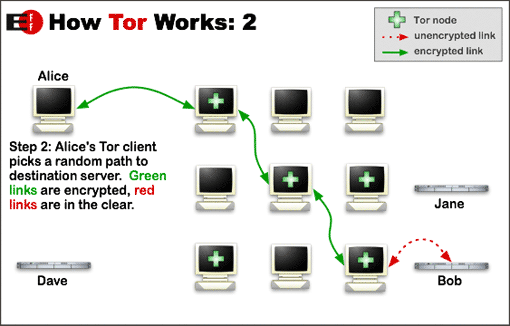
\includegraphics[width=2in]{tor-works}
  \end{center}
  \end{figure}

  \begin{itemize}
  \item Founded by Roger Dingledine and Nick Mathewson (MIT)
  \item Like anonymized U.S. Postal Service.
  \item Protects against privacy attacks.
  \item Most famously motivated by Google search tracking.
  \item Solves privacy.
  \end{itemize}
}

%------------------------------------------------------------------------------
\frame[label=search-nutch]{

  \frametitle{Open Source Search: Nutch}

  \begin{figure}[hbt]
  \begin{center}
  \begin{tabular}{lll}
     
\includegraphics[width=1in]{nutch-logo} &
     
\includegraphics[width=1in]{nutch-robots} &
     
\includegraphics[width=1in]{lucene-logo}
  \end{tabular}
  \end{center}
  \end{figure}

  \begin{itemize}
  \item Founded by (our own) Mike Cafarella and Doug Cutting.
  \item Used publicly by Oregon State University and MozDex (dmoz).
  \item Makes it easy to conduct search research.
  \item Solves privacy and truthfulness.
  \end{itemize}
}

%------------------------------------------------------------------------------
\frame[label=search-future]{

  \frametitle{Speculation on the Future of Search}

  \begin{figure}[hbt]
  \begin{center}
     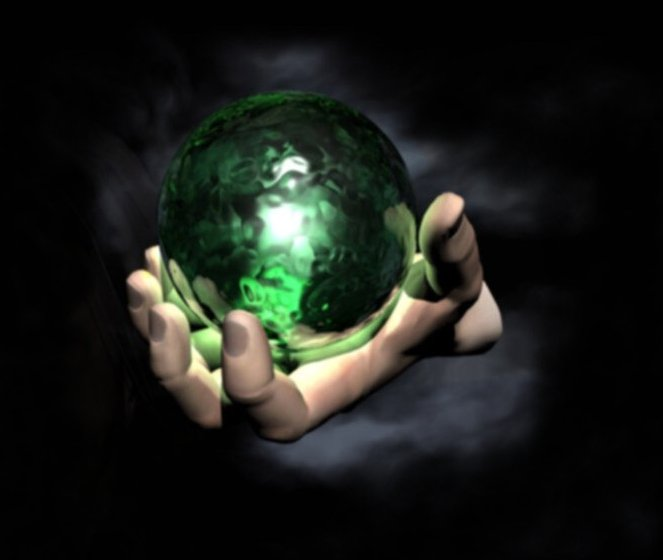
\includegraphics[height=1in]{crystal-ball}
  \end{center}
  \end{figure}

  \begin{itemize}
  \item User crawling instead of link-crawling.
  \item Collaborative searching and tagging.
  \item Peer-to-peer, distributed, social crawling / searching.
  \item Privacy and truthfulness as defaults on new PCs.
  \end{itemize}
}

This is the first section of the article version. In the
presentation, there is a frame containing an overlay. The exact two
slides of this overlay are shown in Figures~\ref{figure-example1}
and~\ref{figure-example2}.

\begin{figure}[ht]
  \begin{center}
    \includeslide{exampleframe<1>}
  \end{center}
  \caption{The first slide. Note the partly covered second item.}
  \label{figure-example1}
\end{figure}

\begin{figure}[ht]
  \begin{center}
    \includeslide{exampleframe<2>}
  \end{center}
  \caption{The second slide. Now the second item is also shown.}
  \label{figure-example2}
\end{figure}


\end{document}



%%% Local Variables: 
%%% mode: latex
%%% TeX-master: "beamerexample2.article"
%%% End: 
